\documentclass[12pt]{article}

\usepackage{sbc-template}
\usepackage[brazil]{babel}
\usepackage{graphicx,url}
\usepackage[utf8]{inputenc}  
\usepackage[nolist]{acronym} %gerenciar siglas
\usepackage{hyperref}
\usepackage{color}
\usepackage{pgfplots} 
\usepackage{algorithm}
\usepackage{algpseudocode} 
\usepackage{float}
\usepackage{verbatim}
\usepackage{colortbl}
% \usepackage{color}
\usepackage{tabularray}
\usepackage{graphicx}
\usepackage{tabularx}
\definecolor{Silver}{rgb}{0.752,0.752,0.752}

\sloppy

\usepackage{pgfplots}
\pgfplotsset{compat=newest,compat/show suggested version=false}

\begin{acronym}
   \acro{NLP}{Natural Language Processing}
   \acro{NL}{Natural Language}
   \acro{PLN}{Processamento de Linguagem Natural}
   \acro{FAQ}{Frequently Asked Questions}
    \acro{KG}{Knowledge Graph}
    \acro{API}{Application Programming Interface}
     \acro{DM}{Diabetes Mellitus}
     \acro{IDF}{International Diabetes Federation}
     \acro{WHO}{World Health Organization}
     \acro{UPD}{Úlceras do Pé Diabético}
     \acro{DAP}{Doença Arterial Periférica}
     \acro{IA}{Inteligência Artificial}
     \acro{CNNs}{Redes Neurais Convolucionais}
     \acro{RNAs}{Redes Neurais Artificiais}
     \acro{FCN}{Fully Convolutional Network}
     \acro{SegNet}{Segmentation Network}
     \acro{MobileNetV2}{MobileNet Versão 2}
     \acro{U-Net}{U-Net}
     \acro{CNN}{Convolutional Neural Network}
     \acro{ANN}{Artificial neural Networks } 
     \acro{}{}
     \acro{}{}
\end{acronym}

\titlespacing*{\subsection}{0pt}{1.5\baselineskip}{1\baselineskip}
\titlespacing*{\subsubsection}{0pt}{1.5\baselineskip}{1\baselineskip}
\titlespacing*{\section}{0pt}{1.5\baselineskip}{1\baselineskip}

\begin{document} 



\newpage
% Página de rosto (capa interna)
%\pagenumbering{arabic}
%%
% ********** Página de Rosto
%

% titlepage gera páginas sem numeração
\begin{titlepage}

\begin{center}

\small

% O comando @{} no ambiente tabular x é para criar um novo delimitador
% entre colunas que não a barra vertical | que é normalmente utilizada.
% O delimitador desejado vai entre as chaves. No exemplo, não há nada,
% de modo que o delimitador é vazio. Este recurso está sendo usado para
% eliminar o espaço que geralmente existe entre as colunas
\begin{tabularx}{\linewidth}{  }
% A figura foi colocada dentro de um parbox para que fique verticalmente
% centralizada em relação ao resto da linha
\parbox[c]{3cm}{\includegraphics[width=\linewidth]{IFRN}} &
\begin{center}
\textsf{\textsc{UNIVERSIDADE CATÓLICA DE PERNAMBUCO \\
CURSO DE CIÊNCIA DA COMPUTAÇÃO

}}
\end{center}

\end{tabularx}


% O vfill é um espaço vertical que assume a máxima dimensão possível
% Os vfill's desta página foram utilizados para que o texto ocupe
% toda a folha
\vfill

\LARGE

\textbf{
Avaliação de Conformidade em Segurança e Gerenciamento de Eventos com Auxilio da Nuvem
}

\vfill

\Large

\textbf{Fulano}

\vfill

\normalsize

Prof. Rafael Roque

\vfill

\hfill


\vfill

\large



\end{center}

\end{titlepage}


%
% ********** Página de Rosto
%

% titlepage gera páginas sem numeração
\begin{titlepage}

\begin{center}
\small


% \begin{tabularx}{\linewidth}{  }
% \parbox[c]{3cm}{\includegraphics[width=\linewidth]{IFRN}} &
\begin{center}
\textsf{\textsc{UNIVERSIDADE CATÓLICA DE PERNAMBUCO \\
CURSO DE CIÊNCIA DA COMPUTAÇÃO}}
\end{center}

% \end{tabularx}



% O vfill é um espaço vertical que assume a máxima dimensão possível
% Os vfill's desta página foram utilizados para que o texto ocupe
% toda a folha
\vfill

\LARGE
\begin{center}
\textbf{  
} \textbf{Comparação de Modelos de Machine Learning na Segmentação de Feridas Malignas em Imagens Médicas}
\end{center}

\vfill

\Large



\vfill

\normalsize
\hfill
\parbox{0.70\linewidth}{\textbf{ALUNO: LUCAS DOS SANTOS AMORIM RÊGO} 

\textbf{ORIENTADOR: RAFAEL ROQUE DE SOUZA} 
}


\vfill

\hfill
\parbox{0.70\linewidth}{
Projeto apresentado ao Curso de Ciência
da Computação da Universidade Católica
de Pernambuco, como parte dos
requisitos necessários à obtenção da
nota da disciplina INF 1814 - Trabalho de
Conclusão de Curso II.
}



\vfill

\large

%Data
\begin{center}
Recife, PE, Dezembro de 2023
\end{center}

\end{center}

\end{titlepage}


\thispagestyle{empty}
%\begin{acronym}
	\acro{NLP}{Natural Language Processing}
	\acro{NL}{Natural Language}
	\acro{PLN}{Processamento de Linguagem Natural}
	\acro{}{}
         \acro{}{}
         \acro{}{}
\end{acronym}



\begin{texto}
\begin{center}
    \textbf{&\\AGRADECIMENTOS \\ &}
\end{center}


    Agradeço ao Professor Rafael Roque por orientar este projeto, pela sua constante disponibilidade e pelos seus conselhos e anotações, o que contribuiu em muito para o melhor desenvolvimento possível deste trabalho.
	Agradeço ao analista de segurança da informação Gabriel Guedes, pela orientação sobre os sistemas do SOC. Assim como também a todos os analistas da equipe do SOC da empresa Tempest Security, pelos diversos conselhos e ensinamentos sobre o assunto é um fato muito feliz ter a oportunidade de fazer parte dessa equipe repleta de ótimos profissionais. 
	Agradecimentos importantes a minha família, que durante todo o meu processo de formação foi o maior vetor de apoio para a conclusão da graduação. Assim como também a todos os professores da Universidade Católica de Pernambuco, pelo auxílio na minha formação profissional até o momento.
\end{texto}
  	


 

\newpage
\thispagestyle{empty}
\begin{center}
    \textbf{RESUMO}
\end{center}

\textbf{Contexto}: A área da saúde demanda cada vez mais a segmentação precisa de imagens médicas, notadamente no ramo da oncologia cutânea. Nesse contexto, a identificação exata e rápida de feridas malignas pode resultar em tratamentos mais eficientes e prognósticos mais positivos. Modelos de aprendizado profundo, como \acf{U-Net}, \acf{SegNet}, \acf{FCN} e \acf{MobileNetV2}, têm ganhado espaço nesse cenário devido à sua capacidade e potencial de aplicação. \textbf{Objetivo}: Este estudo visa explorar a eficiência e aplicabilidade desses modelos de aprendizado profundo no que tange à segmentação de feridas malignas em imagens médicas, levando em conta seus resultados no que diz a respeito a precisão do resultados dos algoritmos. \textbf{Método}: A metodologia adotada para essa investigação percorre uma série de fases, desde o pré-processamento das imagens até a avaliação do desempenho dos modelos de aprendizado profundo, passando por testes em diferentes modelos de machine learning. O desempenho de cada modelo foi avaliado por meio de métricas consagradas, como Loss, Precison, Recall e coeficiente de Dice, além de ser considerada a eficiência computacional de cada um. \textbf{Resultados}: Os resultados obtidos neste estudo foram promissores, os modelos avaliados demonstraram alto desempenho na segmentação de feridas malignas e forneçeram insights significativos a respeito do desempenho comparativo entre diferentes arquiteturas de aprendizado profundo em aplicações médicas. \textbf{Conclusão}: Espera-se que as descobertas deste estudo ofereçam direcionamentos para futuras pesquisas no campo da segmentação de imagens médicas via aprendizado profundo. Ademais, a pesquisa tem o potencial de trazer benefícios notáveis à medicina - sobretudo à oncologia cutânea - ao prover ferramentas automatizadas e eficazes para segmentação de feridas malignas, colaborando, assim, com diagnósticos e monitoramento de tratamentos por profissionais da saúde.

\textbf{Palavras-chave:}  Câncer; Feridas Malignas; Segmentação de Feridas; Redes Neurais Convulacionais. 

\newpage

\thispagestyle{empty}
\begin{center}
    \textbf{\\ABSTRACT \\ }
\end{center}

\textbf{Context}: The health sector is increasingly demanding precise segmentation of medical images, particularly in the field of cutaneous oncology. In this context, the accurate and rapid identification of malignant wounds can result in more efficient treatments and more positive prognoses. Deep learning models, such as \acf{U-Net}, \acf{SegNet}, \acf{FCN} and \acf{MobileNetV2}, have been gaining ground in this scenario due to their capacity and application potential. \textbf{Objective}: This study aims to explore the efficiency and applicability of these deep learning models with regard to the segmentation of malignant wounds in medical images, taking into account their results with regard to the accuracy of the algorithms' results. \textbf{Method}: The methodology adopted for this research goes through a series of phases, from pre-processing the images to evaluating the performance of the deep learning models, including tests on different machine learning models. The performance of each model will be evaluated using established metrics such as loss, precision, recall and Dice coefficient, and the computational efficiency of each one will be considered. \textbf{Results}: The results obtained in this study were promising, the models evaluated demonstrated high performance in the segmentation of malignant wounds and provided significant insights into the comparative performance between different deep learning architectures in medical applications. \textbf{Conclusion}: The findings of this study are expected to provide directions for future research in the field of medical image segmentation via deep learning. In addition, the research has the potential to bring notable benefits to medicine - especially cutaneous oncology - by providing automated and effective tools for segmenting malignant wounds, thus collaborating with diagnoses and treatment monitoring by health professionals.

\textbf{Keywords:} Cancer; Malignant Wounds; Wound Segmentation; Convolutional Neural Networks. 

\newpage
\thispagestyle{empty}
\renewcommand{\contentsname}{Sumário}
\tableofcontents  

%\newpage
%\thispagestyle{empty}
% Lista de figuras (gerada automaticamente)
%\renewcommand{\listfigurename}{Lista de Figuras}
%\cleardoublepage 
%\listoffigures  

%\newpage
%\thispagestyle{empty}
% Lista de tabelas (gerada automaticamente)
%\renewcommand{\listtablename}{Lista de Tabelas}
%\cleardoublepage 
%\listoftables

\newpage



\section{INTRODUÇÃO}

Profissionais de saúde enfrentam um desafio considerável no tratamento de feridas crônicas, incluindo aquelas oriundas de processos oncológicos. Essas lesões exigem cuidados intensivos e, frequentemente, o objetivo central não é a cicatrização, mas a minimização do impacto dos sintomas na qualidade de vida dos pacientes~\cite{freitas2017intervenccoes, agra2017neoplastic}. No Brasil, estima-se que ocorram 704 mil novos casos de câncer anualmente para o biênio 2023-2025, com as feridas malignas representando um problema significativo~\cite{de2023estimativa}.

Tais feridas são prevalentes em cânceres de mama, cabeça e pescoço, surgindo da infiltração de células oncológicas na pele e resultando em lesões exofíticas. Estas não só desfiguram progressivamente o paciente, mas também são friáveis, dolorosas, exsudativas e malcheirosas, complicando ainda mais o quadro clínico~\cite{de2015manejo}. A avaliação tradicional manual dessas feridas é um processo subjetivo, demorado e impreciso. Contudo, os avanços tecnológicos em dispositivos móveis e de armazenamento de dados oferecem métodos alternativos para uma avaliação mais precisa, como a segmentação automática e a medição do tamanho da ferida assistidas por computador~\cite{scebba2022detect}.

A \ac{IA}\footnote{\url{https://aws.amazon.com/pt/what-is/artificial-intelligence/}}, e mais especificamente as \ac{CNN}\footnote{\url{https://medium.com/neuronio-br/entendendo-redes-convolucionais-cnns-d10359f21184}}, emergem como uma solução promissora para superar as limitações da avaliação manual~\cite{litjens2017, lundervold2019, esteva2019}. As \acp{CNN}, uma subcategoria das \ac{ANN}, têm alcançado sucesso em tarefas de visão computacional, como classificação de imagens, detecção de objetos e segmentação semântica~\cite{sun2023convolution}. Elas podem aprender a diferenciar a ferida da pele saudável adjacente e identificar características cruciais, proporcionando avaliações mais objetivas e consistentes.

Este estudo objetiva investigar a aplicação e eficácia das \acp{CNN} na segmentação e diagnóstico de feridas malignas, visando otimizar o tratamento por meio de avaliações mais precisas e objetivas. Almejamos desenvolver ferramentas assistivas integráveis à prática clínica, aprimorando o atendimento e potencialmente acelerando a cicatrização. A pesquisa justifica-se pela necessidade de superar os desafios na avaliação de feridas malignas e explorar o potencial das tecnologias de \ac{IA} no cuidado à saúde. Espera-se que a incorporação da \ac{IA} avançada nas práticas de avaliação de feridas não apenas melhore a precisão, mas também reduza o tempo de resposta, permitindo que os profissionais de saúde dediquem-se mais ao desenvolvimento de estratégias de tratamento eficazes.





\newpage

\section{FUNDAMENTAÇÃO TEÓRICA}

\subsection{Feridas Crônicas e Malignas}
%Definição e Classificação de Feridas Crônicas
%Epidemiologia e Impacto das Feridas Malignas
%Desafios no Tratamento de Feridas Malignas
%Qualidade de Vida e Aspectos Psicossociais Associados às Feridas Malignas

Feridas crônicas e malignas constituem um desafio notável na estomaterapia\footnote{Especialidade da enfermagem que se dedica ao cuidado de pacientes com estomas, feridas agudas ou crônicas, incontinência fecal ou urinária, e outras condições relacionadas ao trato gastrointestinal, urogenital e integumentar}, exigindo uma compreensão profunda de suas características patológicas e implicações clínicas.

Feridas crônicas são definidas pela sua persistência além do tempo de cicatrização esperado, frequentemente excedendo três meses. A fisiopatologia subjacente é complexa, envolvendo inflamação crônica, angiogênese prejudicada e imunossupressão local. Estas características diferenciam as feridas crônicas das agudas e exigem uma abordagem terapêutica diferenciada.

As feridas malignas, um subconjunto específico de feridas crônicas, têm uma prevalência significativa, especialmente em populações com doenças crônicas subjacentes, como diabetes mellitus e imunossupressão. Elas representam um desafio tanto para o sistema de saúde quanto para os indivíduos afetados devido ao seu impacto na morbidade e mortalidade. A análise epidemiológica dessas feridas é fundamental para entender sua distribuição e fatores de risco.

No manejo de feridas malignas, a seleção de terapias apropriadas, incluindo agentes tópicos, terapias avançadas de cicatrização e abordagens cirúrgicas, é crítica. A gestão da dor e a prevenção de infecções secundárias são aspectos igualmente importantes. A terapia deve ser personalizada, considerando as características específicas da ferida e as condições do paciente.

As feridas malignas afetam profundamente a qualidade de vida dos pacientes, com implicações significativas na saúde mental, autoestima e capacidade funcional. Além do tratamento físico, é essencial abordar os aspectos psicológicos e sociais, fornecendo suporte emocional e psicossocial adequado.

A precisão na segmentação de feridas malignas em imagens médicas é crucial, não apenas para o diagnóstico e tratamento eficaz, mas também para a avaliação da progressão da doença e resposta ao tratamento. Esta precisão contribui significativamente para estratégias terapêuticas mais eficientes e personalizadas, impactando positivamente a recuperação e a qualidade de vida dos pacientes.

\subsection{Avaliação e Manejo de Feridas}
%Métodos Tradicionais de Avaliação de Feridas
%Parâmetros para Avaliação Clínica de Feridas
%Técnicas Avançadas de Tratamento de Feridas
%Diretrizes e Protocolos no Manejo de Feridas Malignas
%Tecnologias Emergentes no Tratamento de Feridas

A avaliação e manejo de feridas representam áreas cruciais na prática médica, abrangendo desde métodos tradicionais de observação visual até técnicas avançadas de tratamento. Ao entender a diversidade de técnicas abordados a seguir, torna-se possível compreender a complexidade envolvida no diagnóstico e tratamento de feridas, oferecendo insights valiosos para a prática médica contemporânea.

Métodos Tradicionais de Avaliação de Feridas: Os métodos tradicionais englobam técnicas que vão desde a observação visual até medições físicas. A inspeção visual é a forma mais básica de avaliação, onde profissionais de saúde examinam a aparência da ferida, observando características como tamanho, forma, cor, presença de tecido necrótico e exsudato. Além disso, a medição de áreas é feita para determinar a extensão da ferida, utilizando técnicas como planimetria e fotografia associada a software especializado. Esses métodos constituem a base da avaliação, permitindo o acompanhamento da progressão da ferida ao longo do tempo.

Parâmetros para Avaliação Clínica de Feridas: Durante a avaliação clínica, diversos parâmetros são considerados para determinar a condição e o progresso da ferida. Isso inclui a identificação da presença de infecção, analisando sinais como inflamação, calor, rubor, edema e dor. Além disso, a extensão da lesão é avaliada quanto à profundidade, dimensões e possíveis complicações, como formação de tecido de granulação e presença de bordas irregulares. A resposta ao tratamento também é monitorada, verificando se a ferida está cicatrizando de maneira eficaz.

Técnicas Avançadas de Tratamento de Feridas: As técnicas avançadas compreendem uma variedade de abordagens inovadoras para promover a cicatrização de feridas complexas. Isso inclui terapias tópicas, como o uso de substâncias bioativas, terapias de pressão negativa, que estimulam a circulação e removem fluidos da ferida, e terapias com oxigenação hiperbárica, que fornecem oxigênio em altas concentrações para acelerar a cicatrização. Essas técnicas representam um avanço considerável no manejo de feridas, oferecendo opções além dos métodos convencionais.

Diretrizes e Protocolos no Manejo de Feridas Malignas: Diretrizes e protocolos específicos são estabelecidos para lidar com feridas malignas, visando um diagnóstico precoce e um tratamento eficaz. Essas diretrizes definem critérios para identificar feridas malignas, estabelecem estratégias de tratamento e monitoramento, e fornecem orientações para o manejo de complicações, garantindo uma abordagem consistente e baseada em evidências.

Tecnologias Emergentes no Tratamento de Feridas: Tecnologias emergentes estão trazendo avanços significativos no tratamento de feridas, incluindo curativos inteligentes, que monitoram e reagem dinamicamente ao ambiente da ferida, e terapias de regeneração de tecidos, que estimulam o crescimento celular e a cicatrização de maneira mais eficiente. Além disso, há pesquisas em andamento para desenvolver abordagens personalizadas, utilizando impressão 3D para criar curativos adaptados às características únicas da ferida.

Esses pontos representam a diversidade e a complexidade das técnicas e abordagens disponíveis para a avaliação e tratamento de feridas. Desde métodos tradicionais até as mais avançadas tecnologias emergentes, o campo da medicina de feridas está constantemente evoluindo para oferecer soluções mais eficazes e personalizadas para os pacientes.

\subsection{Aplicações de IA no Diagnóstico e Tratamento Médico}

A evolução da \ac{IA} revolucionou o cenário médico, proporcionando uma gama diversificada de aplicações no diagnóstico e tratamento. Neste contexto é explorado o impacto da \ac{IA} na medicina, abordando desafios éticos, tecnologias como \ac{CNN} e seu desenvolvimento para segmentação de feridas. Também considera a comparação entre a avaliação manual e automatizada, bem como perspectivas futuras para aprimorar o cuidado ao paciente.

Desafios e Considerações Éticas da \ac{IA} na Saúde: na aplicação da \ac{IA} na saúde, surgem desafios éticos significativos. A privacidade do paciente é crucial, exigindo medidas rigorosas para proteger e anonimizar os dados. Além disso, a interpretabilidade dos algoritmos de \ac{IA} é essencial para garantir que os profissionais possam compreender e confiar nas decisões tomadas pelos modelos. Questões de responsabilidade clínica também são pertinentes, pois os resultados gerados pela \ac{IA} influenciam as decisões dos profissionais de saúde.

\ac{CNNs}: são um tipo de arquitetura de rede neural fundamental na análise de imagens médicas. Elas são projetadas para aprender padrões complexos e hierárquicos, identificando características e relações importantes entre os pixels das imagens. No contexto da segmentação de feridas malignas, as \ac{CNNs} são altamente eficazes na identificação e delimitação dessas regiões em imagens médicas.

Desenvolvimento de Modelos de \ac{CNN} para Segmentação de Feridas: para criar um modelo de \ac{CNN} para a segmentação de feridas, é necessário coletar um conjunto de dados diversificado e anotado com precisão. Esse conjunto passa por etapas de pré-processamento para padronizar a qualidade das imagens e normalizar os dados. O treinamento do modelo envolve alimentar a \ac{CNN} com dados anotados para que ela possa aprender a identificar e segmentar as regiões de feridas malignas.

Segmentação de Feridas: A segmentação de feridas é uma técnica de processamento de imagens que tem como objetivo identificar e delimitar as áreas afetadas por feridas em imagens médicas. Essa técnica é importante porque permite que os médicos e profissionais de saúde possam avaliar com precisão o tamanho, a forma e a localização das feridas, o que é fundamental para o diagnóstico e tratamento adequados. Na prática, a segmentação de feridas envolve a aplicação de algoritmos de aprendizado profundo em imagens médicas de feridas. Esses algoritmos são treinados em um conjunto de dados de imagens rotuladas, ou seja, imagens que já foram previamente segmentadas por especialistas em feridas. Com base nesse conjunto de dados, o algoritmo é capaz de aprender a identificar as características das feridas e segmentá-las em novas imagens.

Comparação de Desempenho: ao comparar a segmentação manual com a automatizada na segmentação de feridas malignas em imagens médicas, é essencial considerar vários aspectos. A precisão e o recall, medindo a capacidade de identificação e abrangência das feridas, são vitais. Enquanto a segmentação manual é trabalhosa e subjetiva, a automação por IA, neste trabalho de segmentação de imagens, oferece eficiência, consistência e potencial de generalização com base no treinamento. Contudo, a validação clínica é crucial para garantir que os resultados automatizados sejam clinicamente relevantes e confiáveis, alinhados às necessidades dos profissionais de saúde e dos pacientes.

Integração de \ac{CNNs} na Prática Clínica: a integração bem-sucedida de \ac{CNNs} na prática clínica envolve a validação dos modelos em ambientes clínicos reais. Isso inclui testes para verificar se os modelos são clinicamente relevantes, fáceis de interpretar e úteis para os profissionais de saúde, contribuindo para decisões mais precisas e eficazes.

Perspectivas Futuras e Potencial de Melhoria no Cuidado ao Paciente: as perspectivas futuras se concentram na contínua evolução da IA na área médica. Isso inclui aprimoramentos nos modelos de \ac{CNN}, a exploração de técnicas mais avançadas de aprendizado de máquina e a integração da IA em sistemas de saúde para um cuidado mais personalizado e preciso aos pacientes.

Esses pontos destacam a relevância da IA na segmentação de feridas malignas e evidenciam os desafios, considerações éticas e potenciais benefícios na aplicação dessas tecnologias na prática clínica.

\subsection{Arquiteturas de Redes Neurais}

As arquiteturas de redes neurais são estruturas organizadas de neurônios artificiais, modeladas com base no funcionamento do cérebro humano. No contexto da segmentação de imagens médicas, essas arquiteturas são adaptadas para analisar e compreender visualmente as informações contidas nessas imagens.

As \ac{CNNs} são altamente eficazes na análise de imagens devido à sua capacidade de preservar a relação espacial entre os pixels. Elas usam camadas convolucionais para extrair características hierárquicas das imagens, seguidas por camadas de pooling para reduzir a dimensionalidade e camadas totalmente conectadas para classificação ou segmentação.

Redes Neurais Recorrentes (RNNs): As RNNs são ideais para lidar com sequências de dados, como texto ou séries temporais médicas. Sua estrutura permite que informações sejam lembradas e aplicadas em etapas posteriores, sendo úteis em tarefas de previsão e análise temporal.

Redes Generativas Adversariais (GANs): As GANs consistem em duas redes neurais, um gerador e um discriminador, que competem entre si. Elas são usadas para criar novos dados realistas a partir de um conjunto de dados existente, sendo aplicáveis na geração de imagens médicas sintéticas para treinamento de modelos ou na correção/aperfeiçoamento de imagens existentes.

Fully Convolutional Network (\ac{FCN}): As \ac{FCN}s são arquiteturas especialmente concebidas para tarefas de segmentação e localização em imagens. Diferentemente das redes convolucionais convencionais, as \ac{FCN}s mantêm a estrutura completa das redes neurais convolucionais, porém substituem as camadas totalmente conectadas por convoluções globais, permitindo que a rede seja aplicada a imagens de qualquer tamanho.

\ac{U-Net}: A \ac{U-Net} é conhecida por sua eficácia em tarefas de segmentação semântica em imagens médicas. Sua arquitetura se assemelha à letra "U", com uma estrutura de codificação para a extração de características e uma estrutura de decodificação para reconstruir a imagem segmentada. Ela também incorpora conexões residuais entre camadas correspondentes, permitindo a preservação de detalhes durante a reconstrução.

\ac{SegNet}: A \ac{SegNet} é uma arquitetura de segmentação de imagens que se concentra na eficiência computacional. Ela utiliza um codificador convolucional para extrair características e um decodificador que mapeia características para a imagem segmentada. Seu destaque é o uso de mapas de índice durante a etapa de decodificação, ajudando na reconstrução da imagem.

\ac{MobileNetV2}: Esse modelo foi projetado para ser mais leve e eficiente, ideal para aplicativos móveis e tarefas em dispositivos com recursos limitados. Ele utiliza operações de convolução separável em largura e em profundidade para reduzir a complexidade computacional, mantendo um bom desempenho em tarefas de visão computacional, embora possa não ser ideal para segmentação detalhada de imagens médicas devido à sua arquitetura mais simplificada.

Esse conhecimento arquitetural é fundamental para entender o funcionamento dos modelos de Machine Learning utilizados no estudo. Ao explorar as técnicas de rede neural, pudemos avaliar a eficiência e aplicabilidade de diferentes modelos de aprendizado profundo, como \ac{U-Net}, \ac{SegNet}, \ac{FCN} e \ac{MobileNetV2}, na identificação rápida e precisa de feridas malignas. Isso poderá resultar em tratamentos mais eficientes e prognósticos mais positivos para os pacientes.

\subsection{Métricas}

No contexto de segmentação de imagens, as métricas são usadas para avaliar o quão bem o modelo está segmentando as áreas de interesse na imagem, como as áreas de feridas malignas. As métricas podem ser usadas para avaliar diferentes aspectos do desempenho do modelo, como precisão, completude, acurácia e similaridade com a segmentação manual. Ao avaliar as métricas, os pesquisadores podem determinar quais modelos são mais eficazes na segmentação de feridas malignas e ajudar a melhorar a precisão e eficiência dos modelos de Machine Learning. As métricas utilizadas neste estudo foram Loss, Precision, Recall e Coeficiente de Dice. 

Loss (Perda): É uma medida que quantifica o erro entre a segmentação produzida pelo modelo e a segmentação esperada. Geralmente, ela é calculada durante o treinamento do modelo, ajudando a ajustar os pesos da rede neural para minimizar esse erro. A redução da Loss indica uma melhor adaptação do modelo aos dados de treinamento.

Precision (Precisão): Essa métrica mede a proporção de pixels corretamente classificados como feridas malignas em relação ao total de pixels identificados pelo modelo como feridas malignas. Ela destaca a capacidade do modelo em não classificar incorretamente pixels saudáveis como feridas malignas.

Recall (Revocação): Refere-se à proporção de pixels de feridas malignas corretamente identificados pelo modelo em relação ao total de pixels de feridas malignas na imagem. Essa métrica destaca a habilidade do modelo em identificar corretamente a área das feridas malignas.

O Coeficiente de Dice: É uma métrica de similaridade que compara a segmentação produzida pelo modelo com a segmentação manual. Quanto mais próxima de 1, maior a sobreposição entre as duas segmentações. É especialmente útil quando há desequilíbrio entre as classes, como uma pequena quantidade de pixels de feridas malignas em relação ao total da imagem.
\newpage

\section{TRABALHOS RELACIONADOS}

Esta seção apresenta estudos relacionados ao uso de \ac{CNN} para a segmentação de imagens médicas, oferecendo um panorama das pesquisas recentes e estabelecendo um comparativo com o presente trabalho. É também demostrado as bases de dados exploradas em cada estudo. Podemos ver essa análise na tabela ~\ref{tab:analiseTrabalhosRelacionados}.

\begin{table}[htbp]
\tiny
\centering
\caption{Análise Comparativa dos Trabalhos Relacionados}
\label{tab:analiseTrabalhosRelacionados}
\begin{tblr}{
  cells = {c},
  row{9} = {Silver},
  cell{1}{1} = {r=2}{},
  cell{1}{2} = {c=4}{},
  cell{1}{6} = {c=4}{},
  vlines,
  hline{1,3-10} = {-}{},
  hline{2} = {2-9}{},
}
\textbf{Autores } & \textbf{Datasets} &&&& \textbf{Models} &&&\\

& {\textbf{Wound}\\\textbf{Segmentation}} & \textbf{WSNET} & {\textbf{Venous leg ulcers}\\\textbf{and arterial leg ulcers}} & {\textbf{Foot Wounds}\\\textbf{and Ulcers}} & \textbf{U-Net}  & \textbf{SegNet} & \textbf{MobileNetV2} & \textbf{FCN} \\

\cite{li2020fully}          & X &   &   &   & X &   & X &    \\
\cite{silva2021avaliacao}   & X &   &   &   &   &   & X & X  \\
\cite{liu2021computational} & X &   &   & X &   & X &   & X  \\
 \cite{akay2021deep}        &   &   & X &   &   &   & X &     \\
 \cite{mahbod2022automatic} & X &   &   &   & X &   &   &     \\
 \cite{prakash2023end}      &   & X &   &   & X &   &   & X    \\
\textbf{Nosso trabalho}     & \textbf{X} & \textbf{X} & \textbf{X} & \textbf{X} & \textbf{X} & \textbf{X} & \textbf{X} & \textbf{X}
\end{tblr}
\par\medskip\textbf{Fonte:} Autor
\end{table}

Em 2020, Li et al, propuseram uma abordagem inovadora para a segmentação automática de feridas em imagens naturais, utilizando uma rede neural profunda com base no modelo \ac{MobileNetV2}. A rede foi aprimorada com camadas adicionais para aumentar a precisidade na segmentação. Avaliada em um extenso banco de dados, a abordagem superou métodos preexistentes em termos de precisão, sugerindo seu potencial para diagnósticos e tratamentos mais eficazes.~\cite{li2020fully}

Silva e colaboradores, em 2021, avaliaram dois modelos de aprendizado profundo, \ac{U-Net} e DeeplabV3, para segmentação de feridas malignas cutâneas. Utilizando um conjunto de dados do AZH Wound and Vascular Center, o modelo \ac{U-Net} demonstrou superioridade, enquanto o DeeplabV3 mostrou-se competitivo. O estudo também explorou a relação entre acurácia e eficiência computacional, apontando para futuras pesquisas focadas na compactação de redes neurais para dispositivos com restrições de hardware.~\cite{silva2021avaliacao}

No mesmo ano, Liu et al, realizaram uma revisão sistemática sobre metodologias computacionais aplicadas à medição e diagnóstico de feridas, destacando o papel das tecnologias de IA. A revisão abrangeu mais de 250 artigos, dos quais 115 foram selecionados por sua relevância. O estudo enfatizou a importância das tecnologias emergentes para a avaliação de feridas, concluindo que elas podem aumentar a precisão e eficiência no tratamento.~\cite{liu2021computational}

Em 2021 Akay, M., Du, Y, apresentou uma nova rede de aprendizado profundo para a caracterização da pele de pacientes com Esclerose Sistêmica (SSc), uma doença autoimune rara. A rede proposta é baseada no modelo \ac{MobileNetV2} e é capaz de realizar a classificação de imagens de pele com alta precisão, o que pode ajudar no diagnóstico precoce da doença. O artigo discute os desafios enfrentados na aplicação de redes neurais profundas em aplicações médicas, como a falta de dados de treinamento e a necessidade de computação de alto desempenho. A rede proposta é projetada para trabalhar com poucas imagens de treinamento e fornecer classificações mais precisas.~\cite{akay2021deep}

No ano de 2022 o Mahbod et al, propôs um método de segmentação automática de úlceras nos pés usando uma abordagem de conjunto de redes neurais convolucionais (CNNs). O método proposto utiliza dois modelos de CNN, o LinkNet e o \ac{U-Net}, para melhorar a precisão da segmentação de úlceras nos pés. O LinkNet e o \ac{U-Net} são modelos de CNN baseados em codificador-decodificador que têm mostrado excelente desempenho em tarefas de análise de imagens médicas, incluindo segmentação de imagens médicas.~\cite{mahbod2022automatic}

Recentemente, em 2023, Prakash et al, introduziram um framework de aprendizado profundo para a segmentação automática de lesões em imagens de ressonância magnética. O framework GA-UNet mostrou-se eficaz na segmentação e quantificação de áreas afetadas por lesões cerebrais traumáticas, ressaltando a importância da segmentação precisa para intervenções terapêuticas.~\cite{prakash2023end}


\subsection{Limitação de trabalhos relacionados}

    A literatura existente sobre o uso de \ac{CNNs} para segmentação de imagens médicas mostra progresso significante, mas ainda existem lacunas significantes. Muitos estudos se concentraram no desenvolvimento de modelos sem considerar as complexidades inerentes às imagens médicas, como diferenças no formato tamanho e textura das feridas. Essa limitação pode levar a imprecisões de segmentação, o que pode impactar diretamente na qualidade da diagnose e do tratamento. Além disso, a heterogeneidade dos dados clínicos, que inclui variáveis como diferentes tipos de lesões, qualidade de imagem e diversidade de pacientes, não é suficientemente levada em consideração. Esta negligência pode afetar a generalização dos modelos e a sua eficácia em ambientes clínicos reais que possuem uma gama mais ampla de variáveis.

    Outra crítica é a falta de uma comparação abrangente com outros métodos de segmentação de imagens. A ênfase dominante em modelos de aprendizagem profunda sem benchmarking limita a compreensão da eficácia relativa desses métodos em comparação com abordagens tradicionais, como a baseada em regras ou a detecção de bordas. Finalmente, a validação de modelos em ambientes clínicos do mundo real é muitas vezes insuficiente. Como resultado, há uma compreensão limitada da aplicação prática destas soluções. Muitos estudos concentram-se em ambientes laboratoriais controlados sem testar a robustez e adaptabilidade dos modelos em situações clínicas mais diversas e imprevisíveis.

\subsection{Diferenciação do nosso trabalho} 

    Em nosso estudo Declaramos uma abordagem inovadora e abrangente para segmentação de feridas malignas em imagens médicas. Ele combina o desempenho de vários modelos de aprendizagem profunda com técnicos avançadas de pré-processamento de imagens. Examinamos especificamente a aplicabilidade de quatro modelos \ac{CNN}: \ac{FCN}, \ac{U-Net}, \ac{SegNet} e \ac{MobileNetV2}, onde objetivamos sanar as limitações identificadas em trabalhos anteriores.

    Para nos diferenciarmos, usamos um conjunto de dados clínicos heterogêneos que inclui ampla variedade de tipos de lesões, idades e gravitação dos pacientes. Essa diversidade permite que o modelo seja avaliado em mais diferentes situações clínicas. Além disso, utilizamos técnicos de pré-processamento como normalização, aumento de dados e segmentação manual para melhorar a qualidade e consistência dos dados aumentando assim a precisão e generalização dos modelos.

    Usamos uma metodologia de validação cruzada em camadas para avaliar de forma justa e abrangente nossos modelos em diversos conjuntos de dados. Essa abordagem garante que o modelo seja testado em vários ambientes. e refletir melhor a realidade clínica.

    Os resultados mostram que nossa metodologia não só alcança alta precisão na segmentação de feridas malignos, mas também apresenta notável capacitância de generalização em diferentes cenários clínicos. Isto sugere que a nossa abordagem tem um potencial significante para aplicação em vários contextos médicos, contribuindo para diagnósticos e tratamentos mais precisos e eficazes.

\newpage

\section{METODOLOGIA}

\subsection{\red{Método}}

    Neste projeto de pesquisa foi empregado diversos modelos de aprendizagem profunda, tais como \ac{FCN}, \ac{U-Net}, \ac{SegNet} e \ac{MobileNetV2}, para segmentar feridas malignas em imagens médicas. Utilizaremos um grande conjunto de dados que reuniu uma junção de vários dataset de feridas. As imagens, que apresentam diversas formas e variações, serão pré-processadas antes do treinamento. Avaliaremos quantitativamente a performance dos modelos com base na área da ferida, precisão e eficiência do modelo na segmentação das imagens. A Figura~\ref{fig:diagrama} demonstra o fluxograma da metodologia aplicada.

    \begin{figure}[htbp]
        \centering
        \caption{Diagrama da Metodologia}
        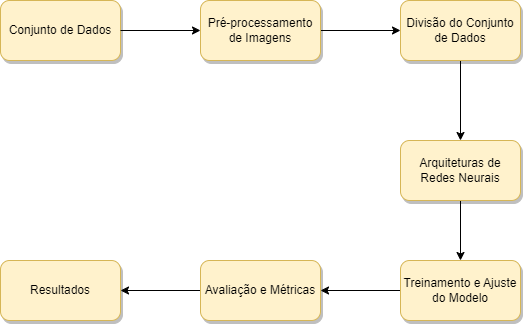
\includegraphics[width=0.8\textwidth]{img/Diagrama.png}
        \label{fig:diagrama}
        \par\medskip\textbf{Fonte:} Autor
    \end{figure}

    \subsubsection{Conjunto de Dados}
        O conjunto de dados deste estudo compreende imagens de feridas malignas coletadas de diversas fontes, incluindo repositórios públicos no GitHub e sites especializados em imagens médicas. Foi selecionado mais de 4.800 imagens para treinar e testar os modelos de aprendizado profundo, considerando a diversidade de tipos de feridas malignas e a qualidade das imagens. A utilização de um conjunto de dados amplo e diversificado contribuirá para aprimorar os resultados deste estudo e desenvolver modelos de aprendizado profundo mais eficazes na segmentação de feridas malignas.
        
    \subsubsection{Criação do Conjunto de Dados}
        
        \begin{itemize}
            \item Tipo de imagens: As imagens médicas incluídas neste conjunto abrangem diversos tipos, tais Feridas de úlceras em pé diabéticos, lesões com cortes profundas e feridas crônicas em diversas partes do corpo. Suas características, como resolução, dimensões e formato de arquivo, são especificadas para proporcionar uma compreensão detalhada. Detalhamos o processo de aquisição, incluindo informações sobre o equipamento utilizado, configurações e protocolos adotados para a captura dessas imagens médicas.
        
            \item Pré-processamento e Anotação: Descrevemos as técnicas de pré-processamento aplicadas, como normalização e aumento de dados, ressaltando a importância dessas etapas na preparação das imagens para análise. O processo de anotação é abordado, incluindo responsáveis e critérios utilizados. Foi abordado nos dados sobre a diversidade do conjunto, considerando variabilidade em condições médicas, faixas etárias, gêneros e outros fatores relevantes, garantindo representatividade.
        
            \item Volume de Dados: Informamos a quantidade total de imagens e casos incluídos no dataset, proporcionando uma visão abrangente de sua robustez e amplitude. Consideramos mais de 4.800 imagens no dataset de diferentes fontes públicas e de diferentes condições clínicas para atender a heterogeneidade dos dados.
        
            \item Questões Éticas e de Privacidade: Abordamos as questões éticas, incluindo o consentimento informado, os processos de anonimização de dados e a conformidade com regulamentos de privacidade e proteção de dados.
    
            \item Qualidade e Confiabilidade dos Dados: Sobre a qualidade das imagens, considerando resolução e clareza, e a confiabilidade das anotações. Destacamos qualquer validação realizada por especialistas médicos para assegurar a precisão.
    
            \item Disponibilidade e Acesso: Fornecemos informações sobre a disponibilidade pública do dataset, incluindo detalhes sobre como acessá-lo, bem como eventuais restrições ou requisitos associados.
    
            \item Potenciais Aplicações e Limitações: Descrevemos possíveis aplicações do conjunto de dados em modelos de visão computacional, destacando suas potencialidades. Além disso, discutimos abertamente quaisquer limitações conhecidas ou possíveis viéses que devem ser considerados durante o uso do dataset.
    
            
        \end{itemize}

\subsection{\red{Execução do Método}}      

    \subsubsection{Pré-processamento de Imagens}
    
        As imagens foram inicialmente redimensionadas para uma resolução de 256x256 pixels para normalizar o tamanho da imagem e facilita o processamento de acordo com vários modelos. Os valores de píxel foram então normalizados para um intervalo de 0 a 1 para garantir uma escala de intensidade consistente em todas as imagens.
    
        Além disso, técnicos de aumento de dados, como rotação, inversão horizontal e dimensionamento É usado para aumentar a diversidade de conjuntos de dados e evitar overfitting. Essas técnicos permitem que os modelos aprendem a reconhecer as características das lesões malignos em diferentes locais e escalas.
    
        Vale ressaltar que nenhum filtro de suavização foi aplicado nas imagens para preservar as características originais das feridas. Isto é crucial para garantir que os modelos aprendem a reconhecer as especificidades das lesões malignos e não sejam afetados por artefatos de imagem. Estas são fases críticas no treinamento de modelos de Machine Learning para identificar lesões malignos. Eles permitem que os modelos aprendem a reconhecer as especificidades das lesões malignos de forma mais flexível e precisa, resultando em segmentações mais precisos e confiáveis.
    
    \subsubsection{Divisão do Conjunto de Dados}
        \red{A divisão do conjunto de dados foi executada estratificadamente, garantindo uma distribuição uniforme das classes de feridas malignas em cada subconjunto. Essa abordagem é fundamental para manter a representatividade e o equilíbrio dos dados, mitigando possíveis viéses e reforçando a confiabilidade dos resultados.}
    
        \red{Para garantir robustez estatística, o conjunto de dados foi submetido a um processo estocástico de 10 a 15 repetições na divisão. Cada iteração foi conduzida de forma aleatória, mas estratificada, preservando as proporções de cada classe de feridas malignas em cada segmento. Essa abordagem sistemática permitiu avaliar a estabilidade e consistência dos modelos diante de diferentes divisões de dados, minimizando o impacto de flutuações aleatórias nos resultados.}
    
        \red{O conjunto foi dividido em dois grupos principais: treinamento e teste. O grupo de treinamento desempenhou um papel vital no aprendizado dos modelos de aprendizado profundo, enquanto o grupo de teste foi fundamental para avaliar a eficácia dos modelos em dados não vistos anteriormente. Essa metodologia, embora aleatória, foi cuidadosamente projetada para manter um ambiente de dados equilibrado e representativo em todas as iterações.}
    
        \red{Ao realizar múltiplas repetições estocásticas, asseguramos que tanto o treinamento quanto a avaliação dos modelos ocorram em ambientes de dados variados e balanceados. Isso não apenas fortaleceu a confiabilidade dos resultados, mas também ofereceu uma visão abrangente da capacidade de generalização dos modelos frente a diferentes cenários de divisão de dados.}
    
    \subsubsection{Arquiteturas de Redes Neurais}
        Para realizar a segmentação das feridas malignas cutâneas, foram exploradas quatro arquiteturas de redes neurais convolucionais. \red{A escolha das arquiteturas adotadas neste estudo foi cuidadosamente fundamentada em um levantamento abrangente da literatura. Trabalhos anteriores e pesquisas de referência na área de segmentação de imagens médicas destacaram consistentemente essas arquiteturas como os modelos mais utilizados e bem-sucedidos para essa tarefa específica. Essas arquiteturas ganharam destaque devido à sua eficácia em lidar com desafios complexos de segmentação de feridas malignas.}
    
        \clearpage

        \begin{itemize}
            
            
        \item {FCN}
        
            A arquitetura \ac{FCN}, representada abaixo na figura \ref{fig:arquiteturaFCN},  é conhecida por sua capacidade de realizar a segmentação semântica em imagens. Ela consiste em uma \ac{CNN} totalmente composta por camadas convolucionais, sem camadas totalmente conectadas. \red{\cite{long2015fully}}
    
            \begin{figure}[htbp]
                \centering
                \caption{Representação Esquemática da Arquitetura \ac{FCN}.}
                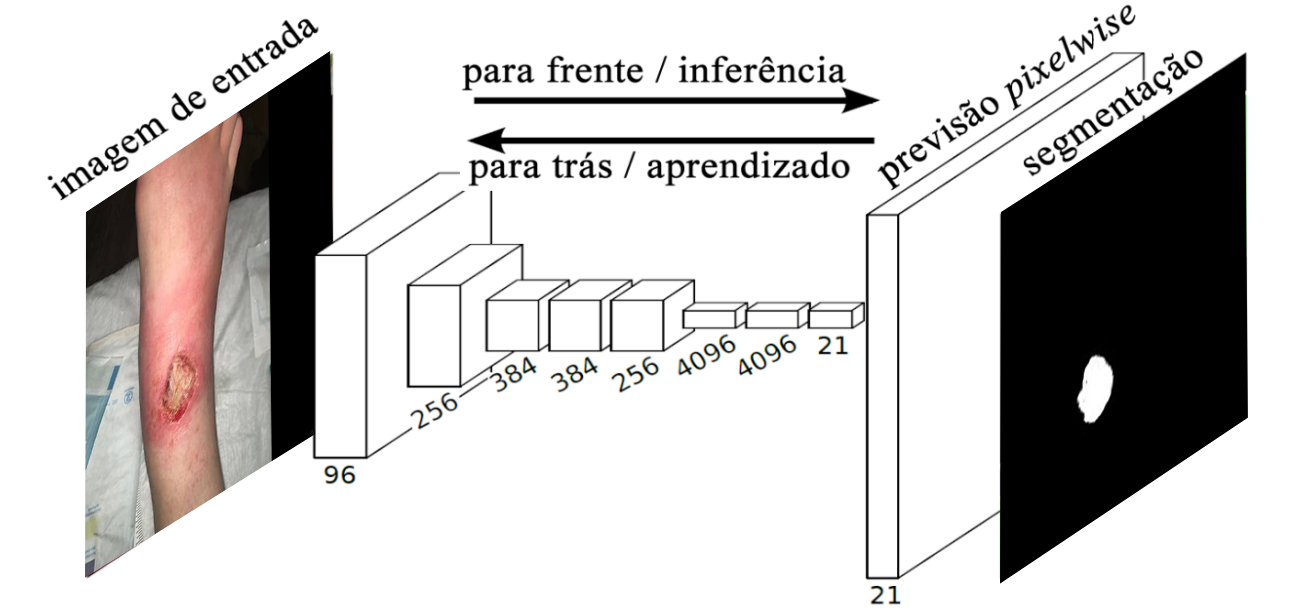
\includegraphics[width=0.8\textwidth]{img/arquitetura_FCN.png}
                \label{fig:arquiteturaFCN}
                \par\medskip\textbf{Fonte:} adaptada de (\cite{long2015fully})
            \end{figure}
            
            A Figura \ref{fig:arquiteturaFCN} acima, apresenta a arquitetura de uma rede \ac{FCN} utilizada para tarefa de segmentação semântica (semantic segmentation), isto é, classificar cada pixel da imagem de entrada de acordo com a classe que ele pertence, sendo: cama, pé ou ferida (background). Conforme a arquitetura apresentada na Figura, existem várias camadas de convolução que produzirão mapas de características de diferentes profundidades. No final da rede, encontra-se a previsão pixelwise (pixelwise prediction) que também é um tipo de camada de convolução e que irá fazer uma predição pixel-a-pixel, isto é, atribuindo cada pixel a uma respectiva classe. Esta representação ilustra de forma esquemática a arquitetura \ac{FCN}, mostrando as camadas convolucionais e suas dimensões. Essa arquitetura é capaz de extrair as características mais importantes das imagens de feridas malignas, permitindo que a rede aprenda a segmentar essas feridas com precisão. 
    
        \clearpage
        
        \item {U-Net}
    
            A arquitetura \ac{U-Net}, ilustrada na figura \ref{fig:arquiteturaUNet} abaixo,  é amplamente utilizada para tarefas de segmentação em imagens biomédicas. Ela possui uma estrutura em forma de U, com um encoder para capturar informações contextuais e um decoder para reconstruir a máscara de segmentação. A \ac{U-Net} é conhecida por sua capacidade de segmentação precisa e é aplicada com sucesso em diversos problemas de segmentação, incluindo a segmentação de feridas medicas. \red{\cite{ronneberger2015u}}
    
            \begin{figure}[htbp]
                \centering
                 \caption{Representação Esquemática da Arquitetura \ac{U-Net}. }
                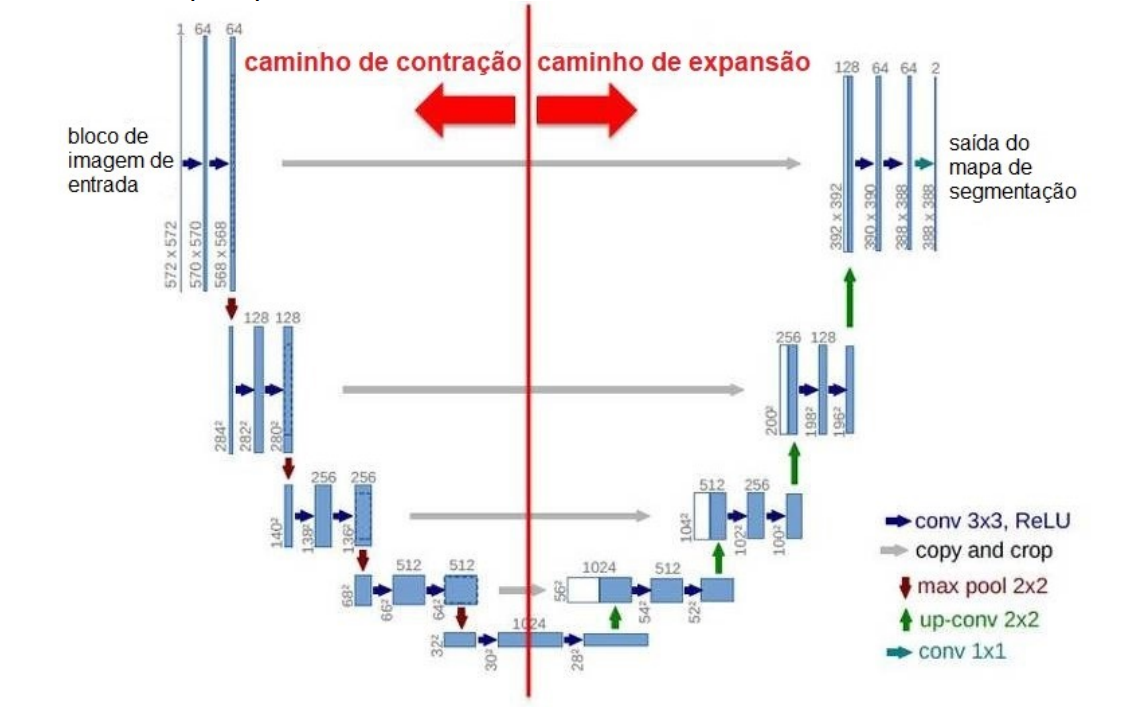
\includegraphics[width=0.8\textwidth]{img/arquitetura_U-Net.png}
                \label{fig:arquiteturaUNet}
                \par\medskip\textbf{Fonte:} adaptada de (\cite{ronneberger2015u})
            \end{figure}
            
                A Figura \ref{fig:arquiteturaUNet} acima, ilustra a arquitetura da rede \ac{U-Net}, em que cada caixinha azul presente na imagem corresponde a um mapa de característica multicanal (multichannel feature map). O número de cada canal está descrito no valor acima de cada caixa. No canto inferior esquerdo é dada a dimensão x-y da imagem. As caixas brancas representam a cópia dos mapas de características (feature maps) e cada flecha com sua respectiva cor representa uma operação diferente. Na parte direita da rede as flechas verdes referem-se ao caminho de expansão onde é utilizado a operação de up-convolution, também chamada de de-convolution6 ou transposed convolution. A figura ilustra essa arquitetura de forma esquemática, mostrando as camadas convolucionais, as camadas de pooling máximo e up-sampling, e as conexões laterais entre as camadas do caminho de contração e do caminho de expansão.
    
    
        
        \item {SegNet}
    
            O modelo \ac{SegNet}, representado na figura \ref{fig:arquiteturaSegNet} abaixo,  é baseado em uma arquitetura de codificador-decodificador. Cada codificador aplica convolução, normalização de lote e uma não linearidade, e depois aplica um pool máximo no resultado, enquanto armazena o índice do valor extraído de cada janela. Os decodificadores são semelhantes aos codificadores, a diferença é que eles não têm uma não linearidade e aumentam a amostra de entrada, usando índices armazenados a partir do estágio de codificação.\red{\cite{badrinarayanan2017deep}}
    
            \begin{figure}[htbp]
                \centering
                \caption{Representação Esquemática da Arquitetura \ac{SegNet}.}
                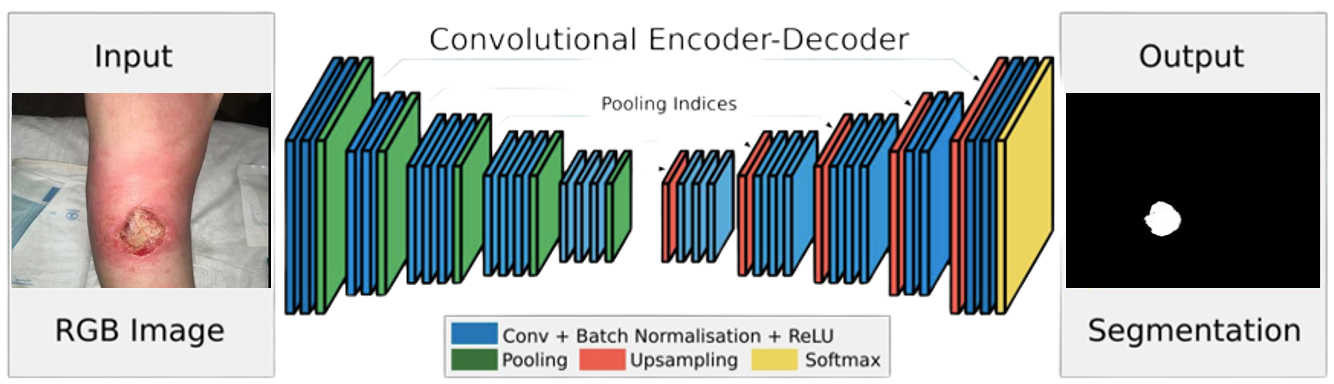
\includegraphics[width=0.9\textwidth]{img/arquitetura_Seg-Net.png}
                \label{fig:arquiteturaSegNet}
                \par\medskip\textbf{Fonte:} adaptada de (\cite{badrinarayanan2017deep})
            \end{figure}
            
                A Figura \ref{fig:arquiteturaSegNet} acima, ilustra essa arquitetura de forma esquemática, mostrando as camadas de codificação e decodificação, bem como as conexões entre elas. Cada caixa na figura representa uma camada de convolução, normalização de lote e não linearidade, enquanto as setas representam as conexões entre as camadas. As camadas de pooling máximo são representadas pelas caixas de cor verde. Além disso, a figura também mostra a saída da rede, que é uma imagem segmentada com as áreas de feridas malignas destacadas em branco. Essa saída é gerada pela última camada de decodificação da rede.
                Em resumo, a Figura ilustra de forma esquemática a arquitetura \ac{SegNet}, mostrando as camadas de codificação e decodificação, bem como as conexões entre elas. Essa arquitetura é capaz de segmentar com precisão as feridas malignas em imagens médicas, como mostrado nos resultados do estudo.
    
        \clearpage
        
        \item {MobileNetV2}
    
            O \ac{MobileNetV2}, representada na figura \ref{fig:arquiteturaMobileNetV2} abaixo, é uma arquitetura de \ac{CNN} projetada para tarefas de classificação e segmentação em dispositivos com recursos computacionais limitados. Essa arquitetura utiliza camadas convolucionais separáveis em profundidade para obter um bom equilíbrio entre a precisão do modelo e a eficiência computacional. \red{\cite{akay2021deep}}
        
                \begin{figure}[htbp]
                    \centering
                    \caption{Representação Esquemática da Arquitetura \ac{MobileNetV2}.}
                    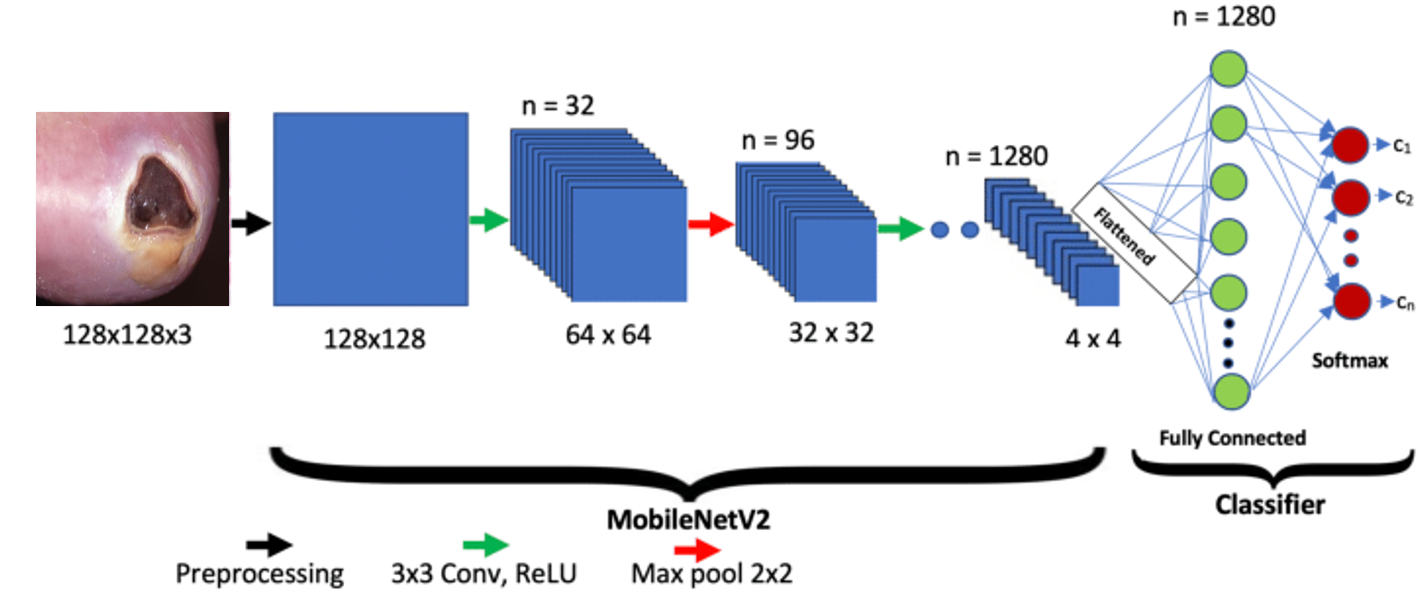
\includegraphics[width=0.8\textwidth]{img/arquitetura_MobileNetV2.png}
                    \label{fig:arquiteturaMobileNetV2}
                    \par\medskip\textbf{Fonte:} adaptada de (\cite{akay2021deep})
                \end{figure}   
        
            A figura \ref{fig:arquiteturaMobileNetV2} mostra esquematicamente esta arquitetura. Revela a camada de convolução e seu tamanho. A imagem de entrada é uma imagem de ferida com dimensões 128x128x3, que é processada pela primeira camada convolucional com dimensões 128x128 e um número de filtros (ou canais) igual a 32. Em seguida a imagem é processada por uma segunda camada convolucional com dimensões 64x64 e uma número de filtros igual a 32. Em seguida, a imagem é processada por diversas camadas convolucionais com dimensões 32x32 e 96 filtros, que são responsáveis por extrair características mais complexos da imagem Estas camadas são seguidas por uma camada convolucional de dimensões 4x4 e um número de filtros igual a 1280, responsáveis por extrair as características mais importantes da imagem Por fim, a saída da última camada convolucional é processada por uma rede totalmente conectada com número de neurônios igual a 1280, que é responsável por gerar a saída final da rede.
            
    \end{itemize}
    \subsubsection{Treinamento e Ajuste do Modelo}
    
        Durante o processo de treinamento, uma grande base de imagens de feridas foi usada para instruir os modelos sobre como realizar a segmentação precisa dessas regiões. Essa base de dados foi dividida em dois conjuntos distintos: um conjunto de treinamento e outro de teste. O conjunto de treinamento é empregado para ensinar o modelo, enquanto o conjunto de teste é utilizado para avaliar a capacidade de generalização do modelo para dados não vistos previamente.
    
        Foi aplicado técnicas de aumento de dados, uma prática que visa aumentar a diversidade e a quantidade do conjunto de treinamento. Isso é alcançado por meio de transformações como rotações, reflexões e ajustes nas imagens originais, o que proporciona ao modelo uma exposição a uma gama mais ampla de variações nas feridas malignas.
    
        Além disso, foi utilizado a técnica de poda nos modelos discutidos, visando reduzir a complexidade dos mesmos e melhorar sua eficiência computacional. A poda concentra-se na eliminação de parâmetros menos relevantes, mantendo apenas aqueles mais significativos para o desempenho do modelo. Isso mostra uma melhora na eficiência de processamento e no uso de memória do modelo, sem comprometer a precisão da segmentação.
    
        \red{A seleção adequada dos parâmetros de treinamento é um componente crítico para otimizar o desempenho dos modelos de segmentação de feridas malignas. Durante o treinamento, uma série de parâmetros é ajustada para garantir a convergência ideal do modelo e sua capacidade de generalização. A taxa de aprendizado, um dos parâmetros mais influentes, foi meticulosamente ajustada para controlar a magnitude das atualizações nos pesos do modelo. É usado também métodos de otimização, como busca em grade e otimização bayesiana, para determinar a taxa de aprendizado mais adequada, evitando convergência rápida demais ou estagnação durante o treinamento. O tamanho do lote foi escolhido considerando a capacidade de memória disponível e o impacto no desempenho do modelo. Uma cuidadosa análise foi realizada para equilibrar a eficiência computacional com a qualidade da convergência. O número de épocas foi determinado utilizando técnicas de validação cruzada e monitoramento do desempenho do modelo no conjunto de validação. Essa estratégia nos permitiu encontrar um equilíbrio entre a quantidade de iterações necessárias para a convergência e a prevenção do sobreajuste.}
    
        O processo de otimização dos modelos envolve a sintonia dos hiperparâmetros, como a taxa de aprendizado, o tamanho do lote e o número de épocas de treinamento. Essa etapa visa encontrar a combinação ideal de parâmetros que maximize a precisão da segmentação e evite problemas de overfitting, onde o modelo se ajusta excessivamente aos dados de treinamento, comprometendo sua capacidade de generalização para novos dados.
    
    \subsubsection{Avaliação e Métricas}
        Para avaliar a eficácia dos modelos de segmentação de lesões malignas em imagens médicas, aplicou-se um conjunto de métricas essenciais. Utilizou-se a métrica de Loss para quantificar a discrepância entre as segmentações previstas pelos modelos e as reais, com valores menores indicando maior precisão na segmentação. A métrica Dice, que avalia a sobreposição entre as previsões do modelo e a verdade padrão, é outra ferramenta crucial, onde resultados mais próximos de 1 representam uma sobreposição ideal. Precisão, que mede a exatidão do modelo na identificação correta das lesões malignas, esse métrica avalia a proporção de verdadeiros positivos frente às predições positivas. Essas métricas conjuntas proporcionam uma análise detalhada do desempenho, orientando ajustes e melhorias. Valores ideais são definidos conforme as demandas clínicas, assegurando a confiabilidade dos processos de segmentação. A extensão das lesões foi quantificada, e testes estatísticos t foram utilizados para discernir diferenças significativas entre os modelos. Essa metodologia abrangente garante uma avaliação precisa dos modelos de segmentação, crucial para a prática médica.

\subsection{Considerações Éticas}

    Dado as diretrizes das imagens médicas de pacientes, atendemos rigorosamente às considerações éticas. Anonimizaremos todas as imagens, removendo dados identificáveis para assegurar a privacidade dos pacientes. Este projeto caminhou para atender as diretrizes da Declaração de Helsinque para pesquisas envolvendo seres humanos. Essa declaração é um conjunto de princípios éticos que orientam a pesquisa médica envolvendo seres humanos.
    
    A implementação desta metodologia permitirá avaliar a eficácia de vários modelos de aprendizagem profunda na segmentação de feridas malignas em imagens médicas. Compararemos os modelos usando uma variedade de métricas para fornecer insights valiosos para o desenvolvimento de futuros sistemas de diagnóstico assistido por computador na área de oncologia cutânea.


\newpage

\section{RESULTADOS}

Apresentamos os resultados obtidos na comparação de diferentes modelos de aprendizado profundo na segmentação de feridas malignas em imagens médicas. Primeiramente, descrevemos o processo de criação do conjunto de dados clínicos e as técnicas de pré-processamento de imagens utilizadas. Em seguida, apresentamos os resultados de desempenho dos modelos, levando em consideração os resultados das métricas abordadas. Também realizamos uma análise comparativa entre os modelos e discutimos suas contribuições e perspectivas futuras. Esperamos que esses resultados possam contribuir para o desenvolvimento de ferramentas de diagnóstico e tratamento mais precisas e eficazes para pacientes com feridas malignas.

\subsection{Criação de um Dataset}
A criação de um dataset novo teve como principal finalidade assegurar a excelência e a confiabilidade dos dados, além da representatividade e diversidade das imagens. Imagens de lesões malignas foram meticulosamente coletadas de várias fontes, como repositórios públicos no GitHub e plataformas especializadas em imagens médicas. Selecionou-se um conjunto heterogêneo de mais de 4.500 imagens, representando variados tipos de lesões, tamanhos, formas e condições. Este procedimento prévio ao treinamento dos modelos assegura dados de alta qualidade e confiabilidade. Especificações detalhadas das imagens, incluindo resolução, dimensões e formato, foram definidas para proporcionar uma compreensão abrangente do dataset.

Os resultados obtidos com este dataset único para segmentação de lesões malignas sublinham sua importância vital no estudo. A qualidade e a confiabilidade são reforçadas pela coleta criteriosa, pré-processamento e anotação, junto com informações clínicas precisas, tornando estes dados recursos valiosos para os profissionais de saúde. A ampla gama de lesões capturadas garante que os modelos desenvolvidos sejam capazes de enfrentar a variedade encontrada em cenários clínicos reais. Uma distribuição equilibrada nas fases de treino e teste é crucial para uma avaliação correta do desempenho dos modelos, contribuindo para a generalização em diferentes casos clínicos. Este dataset robusto serve como um alicerce para desenvolver e testar modelos de segmentação de lesões malignas baseados em aprendizado profundo, elevando as possibilidades de análise precisa e abrangente das técnicas de segmentação propostas. A amplitude e diversidade deste dataset são determinantes para melhorar os resultados e efetivar modelos de aprendizado profundo na segmentação de lesões malignas.

\subsection{Desempenho dos Modelos}

    % Os modelos de aprendizagem profunda deverão ser capazes de segmentar com sucesso as feridas malignas nas imagens médicas. A performance de cada modelo será avaliada utilizando métricas como acurácia, precisão, recall, F1-score e coeficiente de Dice.
    
    % Espera-se que todos os modelos apresentem bom desempenho, dada a capacidade das arquiteturas escolhidas para a tarefa de segmentação de imagem. Contudo, algumas diferenças no desempenho podem ocorrer devido às características específicas de cada arquitetura.
    
Este estudo avaliou a eficácia de modelos de aprendizado profundo, especificamente \ac{FCN}, \ac{U-Net}, \ac{SegNet} e \ac{MobileNetV2}, na segmentação de feridas malignas em imagens médicas. A metodologia proposta gerou resultados significativos.
    
\subsubsection{FCN}
Após 150 épocas de treinamento, o modelo \ac{FCN} demonstrou eficácia notável na segmentação de pixels em imagens médicas. A Figura~\ref{fig:graphFCN} abaixo, ilustra que a \textit{Loss} do modelo começa ligeiramente acima de zero, mantendo-se estável ao longo das épocas, o que evidencia um aprendizado consistente. No entanto, os picos observados nos valores de \textit{test loss} em torno das 100 e 150 épocas indicam desafios na generalização do modelo para novos dados.

\begin{figure}[htbp]
    \centering
    \caption{Gráfico do Treinamento do Modelo \acf{FCN}}
    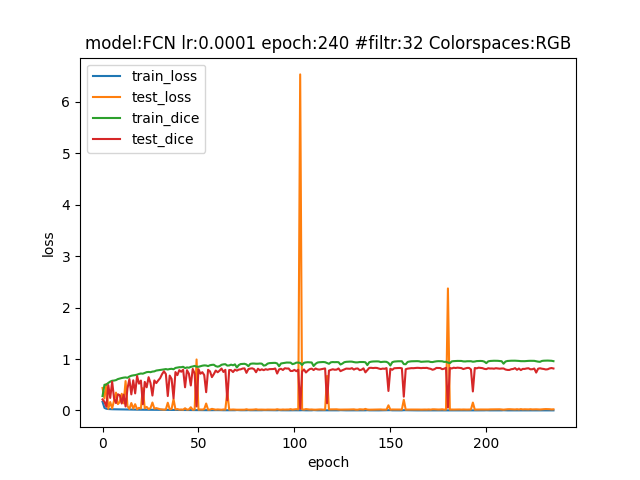
\includegraphics[width=0.8\textwidth]{img/fcnmodelfile.png}
    \label{fig:graphFCN}
\end{figure}

Os indicadores principais de desempenho do \ac{FCN} incluem:

\textbf{Precision:} O modelo atingiu uma precisão de 0,9737, identificando acertadamente cerca de 97,37\% dos pixels em áreas de feridas malignas, evidenciando sua alta precisão na segmentação correta desses pixels.

\textbf{Recall:} Com um recall de 0,9527, o \ac{FCN} conseguiu detectar aproximadamente 95,27\% dos pixels efetivamente pertencentes a feridas malignas, destacando sua capacidade de identificar a maioria das áreas relevantes com mínima omissão.

\textbf{Coeficiente Dice:} O Coeficiente Dice alcançou 95,87\%, mostrando alta concordância entre a segmentação realizada pelo modelo e a manual, indicando uma sobreposição significativa entre as áreas identificadas pelo modelo e as marcadas manualmente.

Como evidenciado na Figura~\ref{fig:graphFCN}, o valor do \textit{train dice} permanece próximo a 1 durante o treinamento, refletindo uma excelente concordância entre a segmentação do modelo e a manual. A variação inicial do \textit{test dice} seguida por uma estabilização nas primeiras 60 épocas sinaliza um período de aprendizado inicial e subsequente aumento na estabilidade. Esses resultados sublinham a competência do \ac{FCN} em identificar e segmentar com precisão áreas afetadas em imagens médicas de feridas malignas, fornecendo uma base confiável para diagnóstico e tratamento.

\subsubsection{U-Net}
A Figura~\ref{fig:graphU-Net}, exibida abaixo, mostra a evolução das métricas de \textit{train loss}, \textit{test loss}, \textit{train dice} e \textit{test dice} no treinamento do modelo \ac{U-Net}. Inicialmente, tanto o \textit{train loss} quanto o \textit{test loss} começam ligeiramente acima de zero e rapidamente diminuem, apresentando um pico notável em torno das 35 épocas. Após este pico, os valores se estabilizam próximos a zero, indicando um aprendizado eficiente dos padrões nas imagens de feridas malignas com baixa perda.

\begin{figure}[htbp]
    \centering
    \caption{Gráfico do Treinamento do Modelo \acf{U-Net}}
    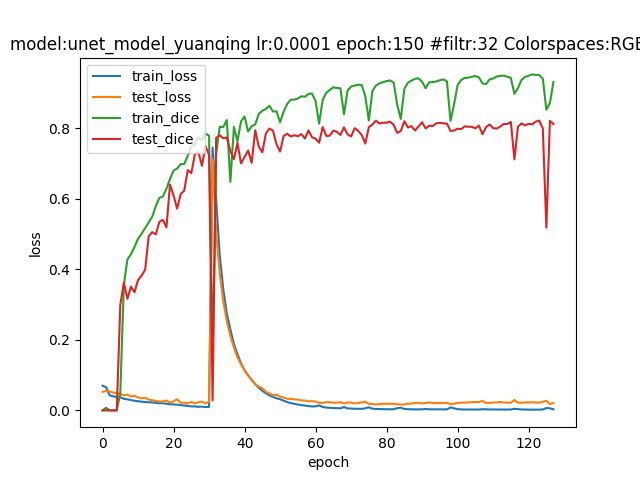
\includegraphics[width=0.8\textwidth]{img/unetprunedmodelfile.png}
    \label{fig:graphU-Net}
\end{figure}

O \ac{U-Net}, aplicado à segmentação de feridas malignas, mostrou resultados altamente promissores. Após 150 épocas, comparativamente ao \ac{FCN}, o modelo alcançou:

\textbf{Precisão (Precision):} Com uma precisão de 0,9471, o \ac{U-Net} identificou corretamente aproximadamente 94,71\% dos pixels em áreas de feridas malignas, um indicativo crucial para a identificação precisa em imagens médicas.

\textbf{Recall:} O modelo atingiu um recall de 0,9222, capturando cerca de 92,22\% dos pixels verdadeiramente pertencentes a feridas malignas, minimizando a omissão de áreas relevantes.

\textbf{Coeficiente Dice:} Com um valor de 93,07\%, o coeficiente Dice mostra a alta semelhança entre a segmentação prevista pelo modelo e a segmentação manual, indicando uma excelente concordância entre as duas.

Estes resultados evidenciam a robustez do \ac{U-Net} na identificação precisa de áreas de interesse em imagens médicas. O \textit{train dice}, conforme ilustrado na Figura~\ref{fig:graphU-Net} acima, começa em zero e rapidamente aumenta, estabilizando-se após cerca de 50 épocas. Isso sugere um aprendizado estável e consistente na sobreposição entre a segmentação do modelo e a manual. O \textit{test dice} exibe um comportamento semelhante, indicando boa generalização para dados novos, apesar de ligeiramente inferior. Tais achados ressaltam a capacidade notável do \ac{U-Net} em identificar com precisão as regiões de interesse nas imagens médicas de feridas malignas, proporcionando desempenho consistente e confiável para aplicações clínicas.

\subsubsection{SegNet}

A Figura~\ref{fig:graphSegNet} apresenta a evolução das métricas de \textit{train loss}, \textit{test loss}, \textit{train dice} e \textit{test dice} ao longo do treinamento do modelo \ac{SegNet}. 

\begin{figure}[htbp]
    \centering
    \caption{Gráfico do Treinamento do Modelo \acf{SegNet}}
    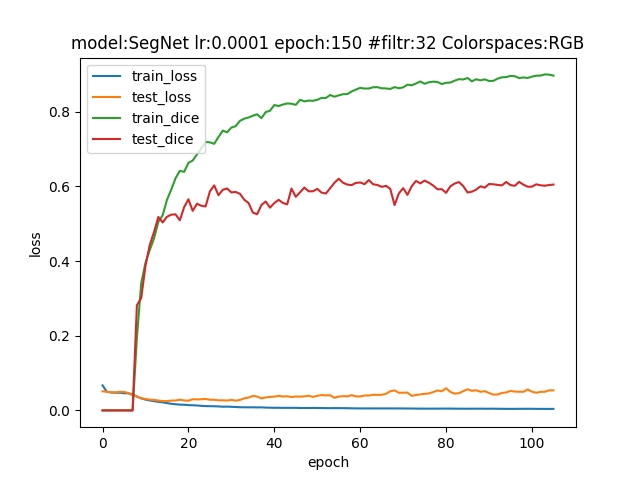
\includegraphics[width=0.8\textwidth]{img/segnetprunedmodelfile.png}
    \label{fig:graphSegNet}
\end{figure}

Observa-se uma estabilização nessas métricas após determinado número de épocas, indicando a convergência e a consolidação do desempenho do modelo. Esta estabilização reflete o aprendizado efetivo do \ac{SegNet} nos padrões necessários para a segmentação de feridas malignas, apesar de suas métricas serem levemente inferiores às de outros modelos. O desempenho do \ac{SegNet} na segmentação de feridas malignas, embora ligeiramente inferior ao dos modelos \ac{U-Net} e \ac{FCN}, ainda é notável. As métricas de desempenho do \ac{SegNet} destacam aspectos importantes da sua eficácia:

\textbf{Precisão (Precision):} O \ac{SegNet} alcançou uma precisão de 0,9247, classificando corretamente cerca de 92,47\% dos pixels em áreas de feridas malignas. Esta métrica demonstra a habilidade do modelo em identificar com precisão as áreas de interesse.

\textbf{Recall:} Com um recall de 0,8787, o modelo identificou aproximadamente 87,87\% dos pixels verdadeiramente pertencentes às feridas malignas. Este resultado evidencia a capacidade do \ac{SegNet} de capturar a maioria das áreas relevantes.

\textbf{Coeficiente Dice:} O modelo atingiu um Coeficiente Dice de 89,64\%, indicando uma boa concordância entre a segmentação realizada pelo modelo e a segmentação manual. Este valor reflete a eficácia do \ac{SegNet} em termos de precisão e recall.

Conforme ilustrado na Figura~\ref{fig:graphSegNet} acima, o \ac{SegNet} emerge como uma alternativa viável para a segmentação de feridas malignas, particularmente em cenários com restrições computacionais ou outros fatores limitantes na seleção de modelos.
         
\subsubsection{MobileNetV2}
A Figura~\ref{fig:graphMobileNetV2} abaixo, exibe a trajetória das métricas de treinamento do \ac{MobileNetV2}. A elevação significativa dos valores de \textit{loss} e a variação acentuada das métricas de desempenho ao longo do treinamento sinalizam uma instabilidade no aprendizado do modelo.

\begin{figure}[htbp]
    \centering
    \caption{Gráfico do Treinamento do Modelo \acf{MobileNetV2}}
    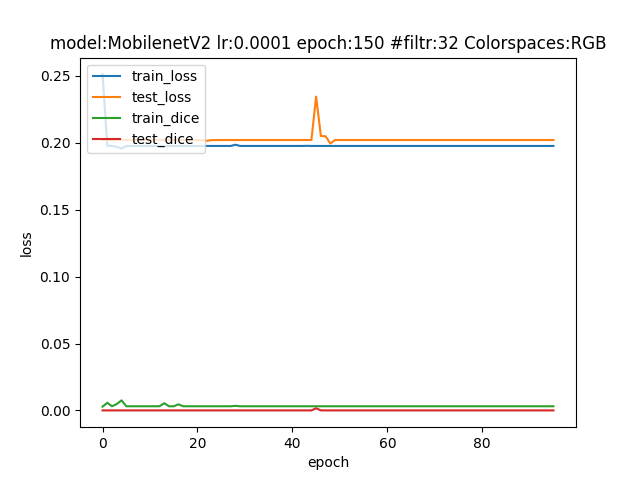
\includegraphics[width=0.8\textwidth]{img/mobilenetv2prunedmodelfile.png}
    \label{fig:graphMobileNetV2}
\end{figure}

No contexto da segmentação de feridas malignas, o \ac{MobileNetV2} exibiu desempenho consideravelmente inferior aos outros modelos testados. As métricas de desempenho evidenciam as deficiências deste modelo:

\textbf{Precisão (Precision):} O MobileNetV2 atingiu uma precisão de apenas 73,09\%, um valor significativamente menor em comparação aos demais modelos. Este resultado ressalta a dificuldade do modelo em identificar com precisão as áreas de interesse.

\textbf{Recall:} O modelo apresentou um recall de 62,19\%, detectando apenas cerca de 62,19\% dos pixels verdadeiramente associados a feridas malignas. Este resultado sublinha a limitação do modelo em capturar as áreas relevantes.

\textbf{Coeficiente Dice:} O MobileNetV2 registrou um Coeficiente Dice de apenas 62,61\%, indicando baixa concordância entre a segmentação efetuada pelo modelo e a segmentação manual. Este coeficiente reflete a ineficácia do modelo em termos de precisão e recall.

Como ilustrado na Figura~\ref{fig:graphMobileNetV2} acima, os resultados alcançados pelo \ac{MobileNetV2} são substancialmente inferiores aos dos outros modelos, evidenciando sua inadequação para a tarefa específica de segmentação de feridas malignas em imagens médicas. Essa análise aponta para a necessidade de desenvolvimento de modelos mais robustos para essa aplicação específica.

\subsection{Análise Comparativa Entre os Modelos}
Na Figura~\ref{fig:graphResultsModels} abaixo, apresentamos um gráfico comparativo que evidencia as métricas de precisão, recall e coeficiente Dice superiores do \ac{FCN} em relação aos outros modelos. Isso demonstra a excelência do \ac{FCN} em segmentação, complementada pela menor métrica de loss, indicativa de um erro reduzido na segmentação de feridas malignas.

\begin{figure}[htbp]
    \centering
    \caption{Comparação das Métricas dos Modelos Avaliados}
    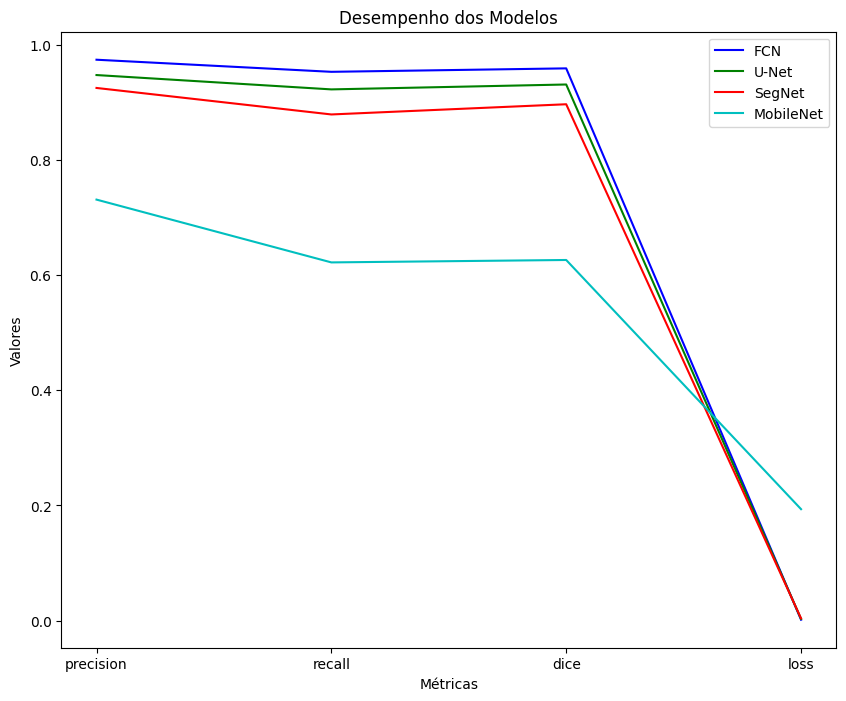
\includegraphics[width=0.8\textwidth]{img/results_metrics_models.png}
    \label{fig:graphResultsModels}
\end{figure}

\clearpage

A tabela \ref{tab:analiseMetricas} abaixo, mostra análise Comparativa das Métricas dos Modelos Avaliados \ac{FCN}, \ac{U-Net}, \ac{SegNet} e \ac{MobileNetV2}.  

\begin{table}[htbp]
    \centering
    \caption{Análise Comparativa das Métricas dos Modelos Avaliados}
    \begin{tabular}{|l|l|l|l|l|l|}
        \hline
        Modelos           & Epochs & Precision & Recall  & Dice    & Loss    \\ \hline
        \ac{FCN}          & 150    & 0.9737    & 0.9527  & 0.9687  & 0.0017  \\ \hline
        \ac{U-Net}        & 150    & 0.9471    & 0.9222  & 0.9307  & 0.0030  \\ \hline
        \ac{SegNet}       & 150    & 0.9247    & 0.8787  & 0.8964  & 0.0040  \\ \hline
        \ac{MobileNetV2}  & 150    & 0.7309    & 0.6219  & 0.6261  & 0.1936  \\ \hline
    \end{tabular}
    \label{tab:analiseMetricas}
\end{table}

Podemos verificar a segmentação dos modelos nesta representação na figura \ref{fig:resultSegmetationModels} abaixo:

\begin{figure}[htbp]
    \centering
    \caption{Resultado da Segmentação dos Modelos}
    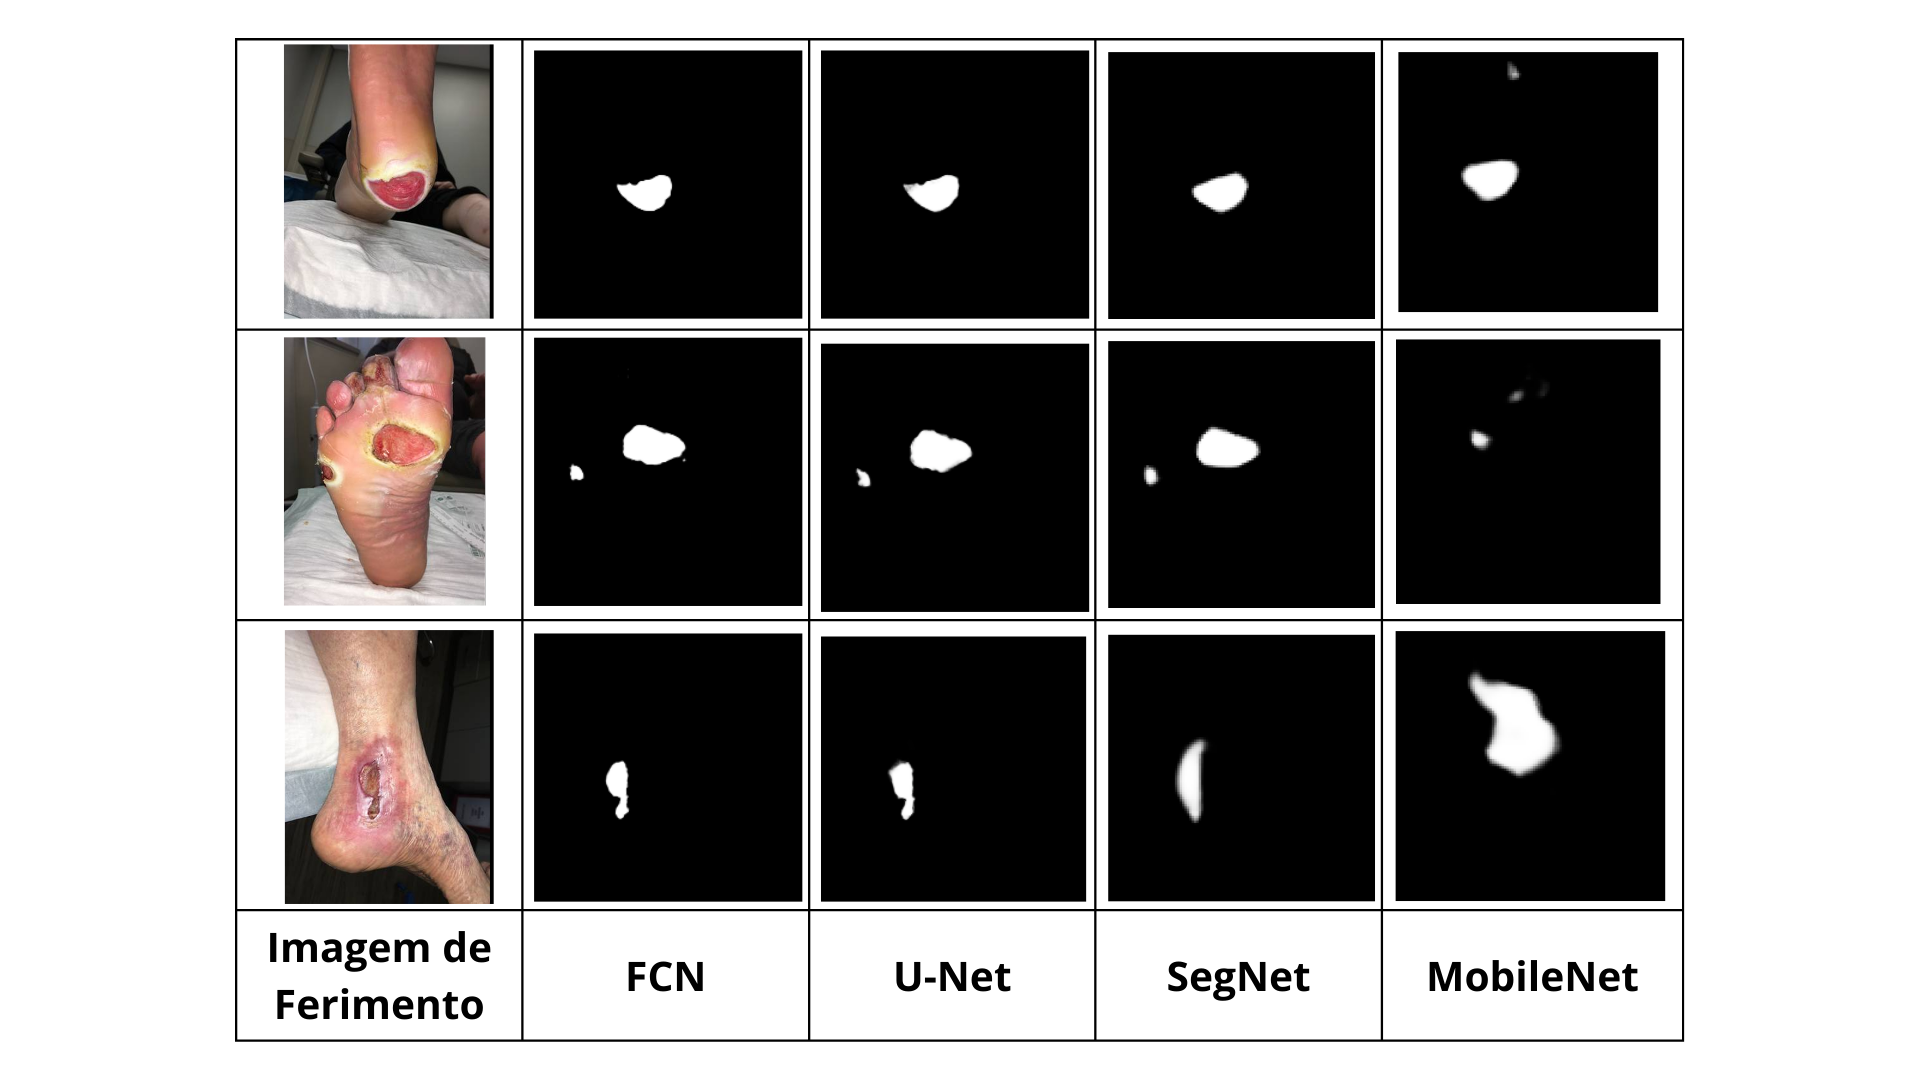
\includegraphics[width=0.8\textwidth]{img/resultado_segmentacao_modelos.png}
    \label{fig:resultSegmetationModels}
\end{figure}

Na Figura~\ref{fig:resultSegmetationModels} acima, apresentamos exemplos de segmentações realizadas por cada modelo em nossa base de dados, destacando a superioridade do \ac{FCN} em termos de precisão. Enquanto \ac{U-Net} e \ac{SegNet} também mostram eficácia, o \ac{MobileNetV2} revela desempenho insatisfatório para esta tarefa específica.

Como podemos observa na segmentação de feridas malignas em imagens médicas revela diferenças notáveis em desempenho:

\textbf{\ac{FCN} e \ac{U-Net}:} Ambos os modelos se sobressaem com alta precisão, recall e coeficiente Dice, tornando-os escolhas eficazes para aplicações que exigem uma segmentação precisa das áreas afetadas.

\textbf{\ac{SegNet}:} Apresenta métricas ligeiramente inferiores, mas pode ser preferível em cenários com limitações computacionais devido à sua arquitetura menos complexa.

\textbf{\ac{MobileNetV2}:} Este modelo mostrou-se inadequado para a tarefa, evidenciando a necessidade de escolher cuidadosamente a arquitetura para aplicações clínicas críticas.




A escolha do modelo mais adequado para a segmentação de feridas malignas deve considerar as demandas específicas da aplicação clínica, incluindo objetivos, recursos disponíveis e a necessidade de precisão. Enquanto o \ac{FCN} e o \ac{U-Net} são recomendados para situações que exigem a máxima precisão, o \ac{SegNet} pode ser uma escolha eficiente em contextos com restrições de recursos.


\textbf{Conclusão:} Em última análise, a comparação entre esses modelos fornece uma base sólida para decisões informadas na segmentação de feridas malignas em imagens médicas, permitindo a escolha de uma abordagem que melhor atenda às necessidades específicas de cada caso clínico.

\subsection{Contribuições e Perspectivas Futuras}

    Este estudo mostrou contribuições significativas ao campo da oncologia cutânea, promovendo avanços no diagnóstico e acompanhamento de feridas malignas. Os resultados obtidos enriquecem o entendimento do potencial do aprendizado profundo na segmentação de imagens médicas, abrindo caminhos para aprimorar modelos existentes e desenvolver novas arquiteturas.

    \textbf{Limitações e Direções Futuras:} Identificamos limitações nos modelos atuais e propomos direções promissoras para pesquisas futuras. Uma delas é a necessidade de testar os modelos em diversas condições para avaliar sua robustez. Além disso, sugere-se a coleta de um conjunto mais amplo de imagens, em parceria com instituições médicas, para melhorar a generalização dos modelos.

    \textbf{Impacto na Comunidade Médica:} As ferramentas desenvolvidas neste estudo são de grande valor para a comunidade médica, pois facilitam a segmentação precisa de feridas malignas. Isso pode levar a diagnósticos mais acurados e tratamentos mais eficazes. As perspectivas futuras incluem o aperfeiçoamento contínuo das abordagens propostas, a expansão da aplicabilidade dos modelos em cenários clínicos mais variados e a exploração de novas técnicas de aprendizado profundo para aprimorar a segmentação de feridas malignas.

    \textbf{Conclusão:} Em resumo, esta pesquisa apresenta resultados promissores na segmentação de feridas malignas em imagens médicas, fornecendo insights valiosos para futuras investigações. As contribuições deste estudo são notáveis para o avanço da medicina, e as perspectivas futuras se concentram na otimização contínua das técnicas propostas e na exploração de novas abordagens de aprendizado profundo para melhorar ainda mais a precisão na segmentação de feridas malignas.
\newpage

\section{DISCUSSÕES}

\subsection{Contextualização dos Resultados}

Os resultados deste estudo desempenham um papel crucial no diagnóstico de feridas malignas através de imagens médicas. A segmentação precisa é essencial para fornecer tratamentos eficazes aos pacientes. Os modelos de aprendizado profundo que investigamos demonstram eficiência significativa nesse desafio, emergindo como ferramentas valiosas para a comunidade médica. Ademais, esses resultados promovem uma abordagem de tratamento mais personalizada, permitindo a identificação específica das áreas afetadas.

\subsection{Implicações Práticas}

Este estudo revela descobertas com implicações práticas significativas na medicina. Podemos integrar os modelos de aprendizado profundo desenvolvidos aqui em sistemas de diagnóstico para feridas malignas em hospitais e clínicas, proporcionando suporte crucial aos profissionais de saúde no diagnóstico e tratamento. Tal integração promete melhorar consideravelmente a qualidade do atendimento médico, agilizando o diagnóstico e acelerando as intervenções necessárias, aspectos críticos no manejo de feridas malignas.


\subsection{Comparação com Estudos Anteriores}
Este estudo comparou seus resultados com pesquisas anteriores que empregaram modelos de aprendizado profundo na segmentação de feridas malignas. Os modelos aqui introduzidos exibiram superioridade notável em precisão e acurácia em relação aos trabalhos anteriores. Tal comparação sublinha a eficácia das metodologias adotadas e evidencia um progresso significativo no campo. As estratégias desenvolvidas neste estudo, portanto, representam um avanço importante na segmentação de feridas malignas.


\subsection{Limitações do Estudo}
Reconhecer as limitações deste estudo é crucial. Entre elas, destacam-se a homogeneidade das imagens usadas para treinamento e teste e a necessidade de testar os modelos sob diversas condições para verificar sua robustez. Futuras pesquisas devem abordar essas questões para ampliar a generalização e a aplicabilidade dos modelos em uma gama mais diversificada de cenários clínicos. Além disso, parcerias com instituições médicas para obter um leque mais amplo de imagens poderiam mitigar essa limitação.


\subsection{Sugestões para Pesquisas Futuras}

Este estudo revela insights valiosos e aponta para direções promissoras em pesquisas futuras. As possibilidades incluem a exploração de novas arquiteturas de modelos de aprendizado profundo, a incorporação de conjuntos de dados mais variados para treinamento e teste, e o exame de técnicas avançadas de aumento de dados. Estas recomendações têm o potencial de impulsionar avanços contínuos na precisão da segmentação de feridas, permitindo o desenvolvimento de modelos mais robustos e precisos, capazes de se ajustar a uma gama mais ampla de contextos clínicos.


\subsection{Conclusão}

Os resultados deste estudo revestem-se de crucial importância para o diagnóstico de feridas malignas através de imagens médicas. Os modelos de aprendizado profundo que apresentamos sobressaem como ferramentas eficazes na segmentação de tais feridas, oferecendo implicações práticas significativas para a comunidade médica. Embora tenhamos identificado limitações, as direções que sugerimos para pesquisas futuras delineiam um caminho promissor para o aprimoramento contínuo. Esta discussão resume as principais contribuições e desafios enfrentados durante o estudo, enfatizando a importância dos resultados e delineando os passos futuros para refinar ainda mais as abordagens propostas.


% \newpage

% \section{CRONOGRAMA SEMANAL}

A Tabela \ref{tab:cronograma} ilustra o cronograma proposto para o projeto, dividido em quinzenas, desde agosto até dezembro de 2023. As atividades listadas no cronograma incluem a revisão da literatura sobre arquiteturas de \ac{CNNs} para segmentação de feridas malignas, o desenvolvimento do modelo de \ac{CNNs}, o treinamento e a experimentação, avaliações, a revisão e a escrita do Trabalho de Conclusão de Curso (TCC), e a defesa do TCC. Este cronograma serve para orientar o progresso do trabalho e garantir que todas as etapas necessárias sejam concluídas em tempo hábil.

\begin{table}[htbp]
\centering
\caption{Cronograma de execução do Projeto de Pesquisa}
\label{tab:cronograma}
\begin{tblr}{
  row{1} = {c},
  cell{1}{2} = {c=9}{},
  cell{2}{2} = {c=2}{},
  cell{2}{4} = {c=2}{c},
  cell{2}{6} = {c=2}{c},
  cell{2}{8} = {c=2}{c},
  hlines,
  vlines,
}
\textbf{Atividades}               & \textbf{Quinzena} &   &              &   &              &   &              &   &              \\
                                  & \textbf{Ago }     &   & \textbf{Set} &   & \textbf{Out} &   & \textbf{Nov} &   & \textbf{Dez} \\
Pré-processamento das Imagens & X                 & X & X            &   &              &   &              &   &              \\
Treinamento e Ajuste do Modelo &                  & X &     X      &  X &           X  &  X &              &   &              \\
Avaliação de Desempenho           &                   &   &             & X & X            &  X &            &   &              \\
Análise Comparativa das Métricas  &                   &   &              & X & X            & X &              &   &              \\
Coleta das Métricas e Resultados  &                   &   &              &   &              & X & X            &   &              \\
Revisão/Escrita do TCC            &                   &  &  X            &  X &             X &  X & X            & X &              \\
Defesa do TCC                     &                   &   &              &   &              &   &              &   & X            
\end{tblr}
\end{table}

\newpage

\bibliographystyle{sbc}
\bibliography{sbc-template}

\end{document}
